\section{Results}

This section presents the main results of the study. First, we compare the
performance of the evaluated models. Then, we analyze the classification
performance of the best model  through confusion matrices, ROC-AUC curves, and
class-wise metrics. Figures for the rest of the models can be found attached in
Annexes.

\subsection{Model Comparison}

Table \ref{tab:tab3} presents a detailed comparison of four classification
models—KNN, RF, SVM, and ANN—under three validation strategies: Baseline,
Simple Split, and Stratified K-Fold.

Under the Baseline setting, where no validation is applied, overall performance
is low. KNN and SVM both show an accuracy of 0.35 with wide 95\% confidence
intervals (0.14, 0.56), while ANN performs worst with 0.20 (0.02, 0.38),
indicating instability. RF performs noticeably better, reaching 0.75 (0.56,
0.94), clearly higher than the others.

In the Simple Split strategy, all models improve. KNN and ANN both reach 0.70
(0.50, 0.90), and SVM increases to 0.60 (0.39, 0.81). RF remains the top
performer with 0.80 (0.62, 0.98). This suggests that even a basic train-test
split brings performance gains over the baseline.

With Stratified K-Fold, performance increases further and the ranking among
models shifts. SVM now achieves the highest accuracy at 0.85 with a relatively
narrow interval (0.69, 1.00), showing more consistent performance. KNN and
Random Forest both reach 0.80 with the same interval (0.62, 0.98), while ANN
remains at 0.70 (0.50, 0.90). The intervals across models are generally
narrower here, which may point to more reliable estimates under this strategy.

\begin{table}[H]
	\centering
	\caption{Performance metrics under different validation strategies (Baseline, Simple
		Split, and Stratified K-Fold). KNN $=$ k-Nearest Neighbors, RF $=$ Random
		Forest, SVM $=$ Support Vector Machine, ANN $=$ Artificial Neural Network.}
	\label{tab:tab3}
	\begin{adjustbox}{max width=0.99\textwidth}
		\begin{tabular}{llcccc}
			\toprule
			\textbf{Split} & \textbf{Metric}    & \textbf{KNN}      & \textbf{RF}                & \textbf{SVM}               & \textbf{ANN}      \\
			\midrule
			\multirow{5}{*}{Baseline}
			               & Accuracy (95\% CI) & 0.35 (0.14, 0.56) & \textbf{0.75 (0.56, 0.94)} & 0.35 (0.14, 0.56)          & 0.20 (0.02, 0.38) \\
			               & Precision (macro)  & 0.45              & \textbf{0.74}              & 0.57                       & 0.04              \\
			               & Recall (macro)     & 0.35              & \textbf{0.75}              & 0.35                       & 0.20              \\
			               & F1 Score (macro)   & 0.38              & \textbf{0.73}              & 0.35                       & 0.07              \\
			               & ROC-AUC (macro)    & 0.72              & \textbf{0.84}              & 0.50                       & 0.50              \\
			\midrule
			\multirow{5}{*}{Simple}
			               & Accuracy (95\% CI) & 0.70 (0.50, 0.90) & \textbf{0.80 (0.62, 0.98)} & 0.60 (0.39, 0.81)          & 0.70 (0.50, 0.90) \\
			               & Precision (macro)  & 0.78              & \textbf{0.82}              & 0.73                       & 0.73              \\
			               & Recall (macro)     & 0.70              & \textbf{0.80}              & 0.60                       & 0.70              \\
			               & F1 Score (macro)   & 0.71              & \textbf{0.80}              & 0.60                       & 0.69              \\
			               & ROC-AUC (macro)    & 0.88              & \textbf{0.95}              & 0.87                       & 0.91              \\
			\midrule
			\multirow{5}{*}{K-Fold}
			               & Accuracy (95\% CI) & 0.80 (0.62, 0.98) & 0.80 (0.62, 0.98)          & \textbf{0.85 (0.69, 1.00)} & 0.70 (0.50, 0.90) \\
			               & Precision (macro)  & 0.83              & 0.83                       & \textbf{0.89}              & 0.80              \\
			               & Recall (macro)     & 0.80              & 0.80                       & \textbf{0.85}              & 0.70              \\
			               & F1 Score (macro)   & 0.80              & 0.80                       & \textbf{0.85}              & 0.67              \\
			               & ROC-AUC (macro)    & 0.95              & 0.95                       & \textbf{0.98}              & 0.95              \\
			\bottomrule
		\end{tabular}
	\end{adjustbox}
\end{table}

\subsection{Confusion Matrix and ROC-AUC Curve}

Selecting our best-performing model—SVM evaluated using the stratified K-Fold
strategy—we observe robust and well-balanced performance across all five
cardiac conditions, as shown in Figure \ref{fig:fig3}.

The confusion matrix shows perfect classification for all cases of MINF and RV.
On the other hand, DCM and HCM are misclassified as MINF, which may indicate
that the model tends to associate overlapping structural features from these
cardiomyopathies with those of MINF. This is in line with prior observations by
Bellotti et al. \cite{bellotti2002}, who noted that DCM and HCM can exhibit
morphologic characteristics that may overlap not only with each other but also
with features observed in MINF, particularly in early or atypical stages. One
NOR case is also misclassified as RV, but overall the predictions remain highly
accurate. Interestingly, the strong performance of the RV class stands out,
especially considering that the right ventricle is often described as more
difficult to assess and characterize due to its complex geometry, thin walls,
and highly variable contraction patterns \cite{sievers2014}.

The ROC-AUC curves reinforce these results, with all classes achieving values
above 0.94. Notably, RV reaches 1.00, while DCM, NOR, and HCM each exceed 0.97.

\begin{figure}[H]
	\begin{center}
		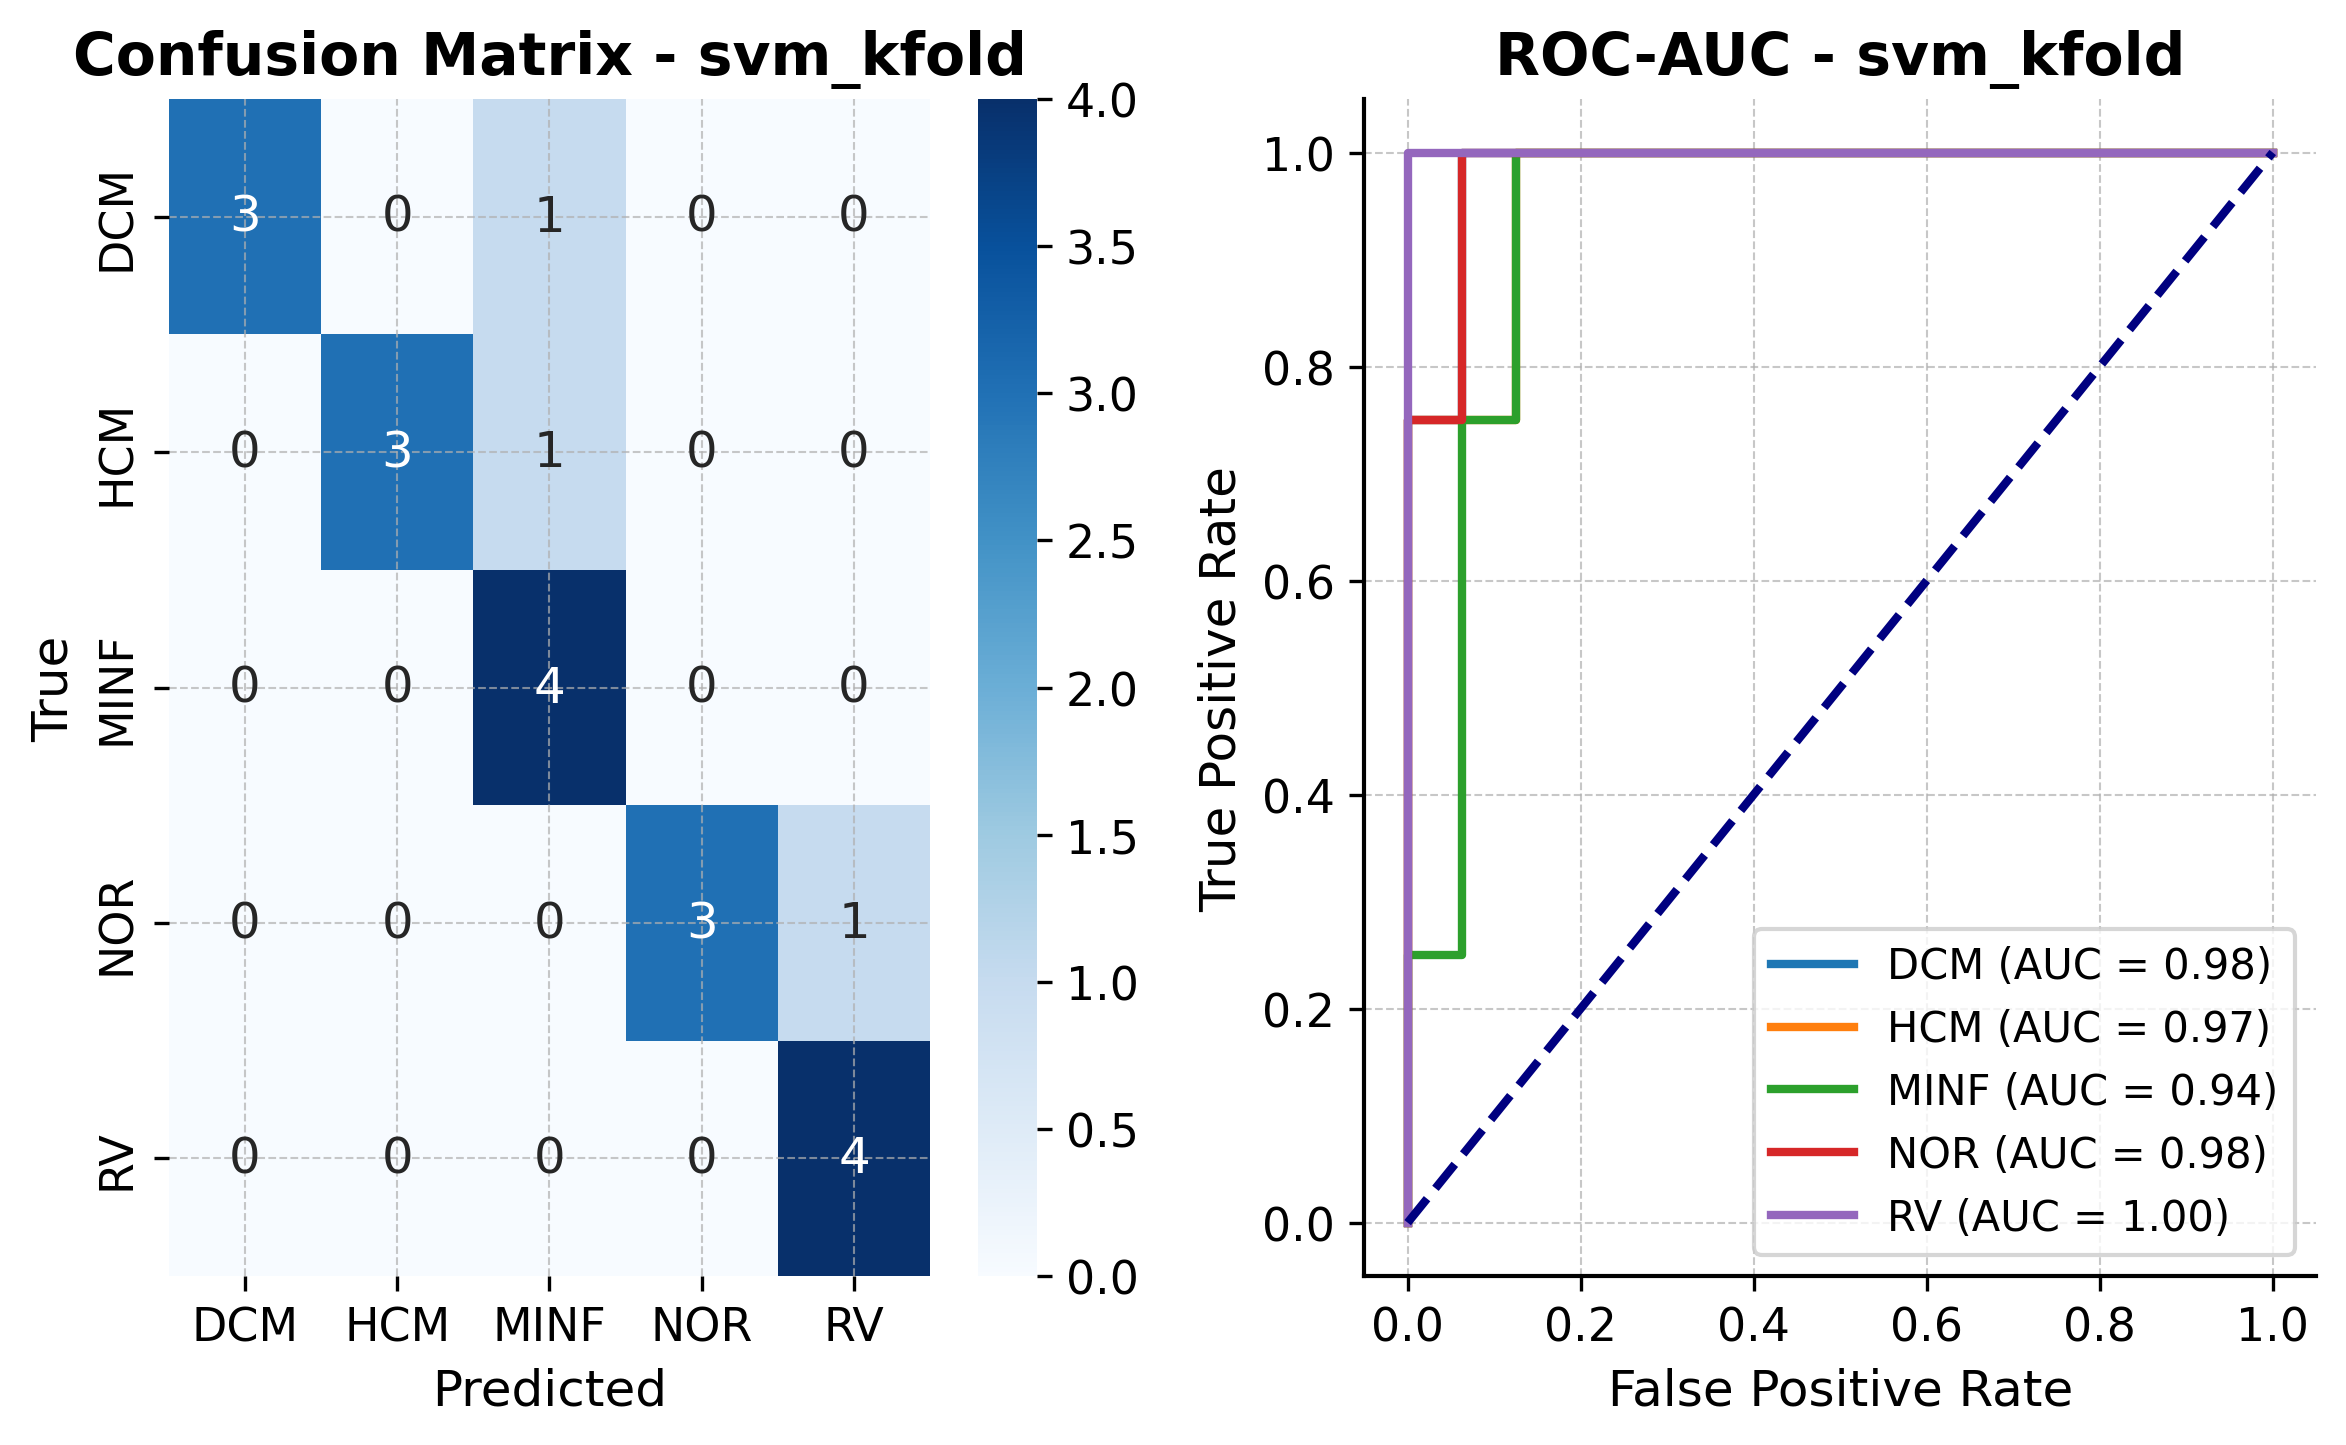
\includegraphics[width=0.99\textwidth]{../images/metrics/svm/svm_kfold_metrics.png}
	\end{center}
	\caption{Confusion matrix and ROC curves for the Support Vector Machine (SVM)
		model trained with Stratified K-Fold cross-validation. DCM $=$ Dilated
		Cardiomyopathy, HCM $=$ Hypertrophic Cardiomyopathy, MINF $=$ Myocardial
		Infarction, NOR $=$ Normal, RV $=$ Right Ventricular abnormality.}
	\label{fig:fig3}
\end{figure}

\subsection{Class-wise Metrics}

To ensure that no single class disproportionately influenced the overall
performance metrics, we analyzed class-specific precision, recall, and
F1-scores, as presented in Figure \ref{fig:fig4}.

DCM and HCM show high precision but lower recall, suggesting that the model is
selective when assigning these labels and may miss some true cases. Both
classes were previously misclassified as MINF, indicating potential overlap in
their structural features. Therefore, even though MINF achieves perfect recall,
it shows lower precision, reflecting a tendency to attract false positives. NOR
shows balanced performance, with only a slight drop in recall due to one
misclassified case. RV maintains strong and consistent values across all
metrics, indicating that it was both reliably identified and not confused with
other classes. This final analysis further supports the patterns observed in
the confusion matrix and ROC-AUC curves.

\begin{figure}[H]
	\begin{center}
		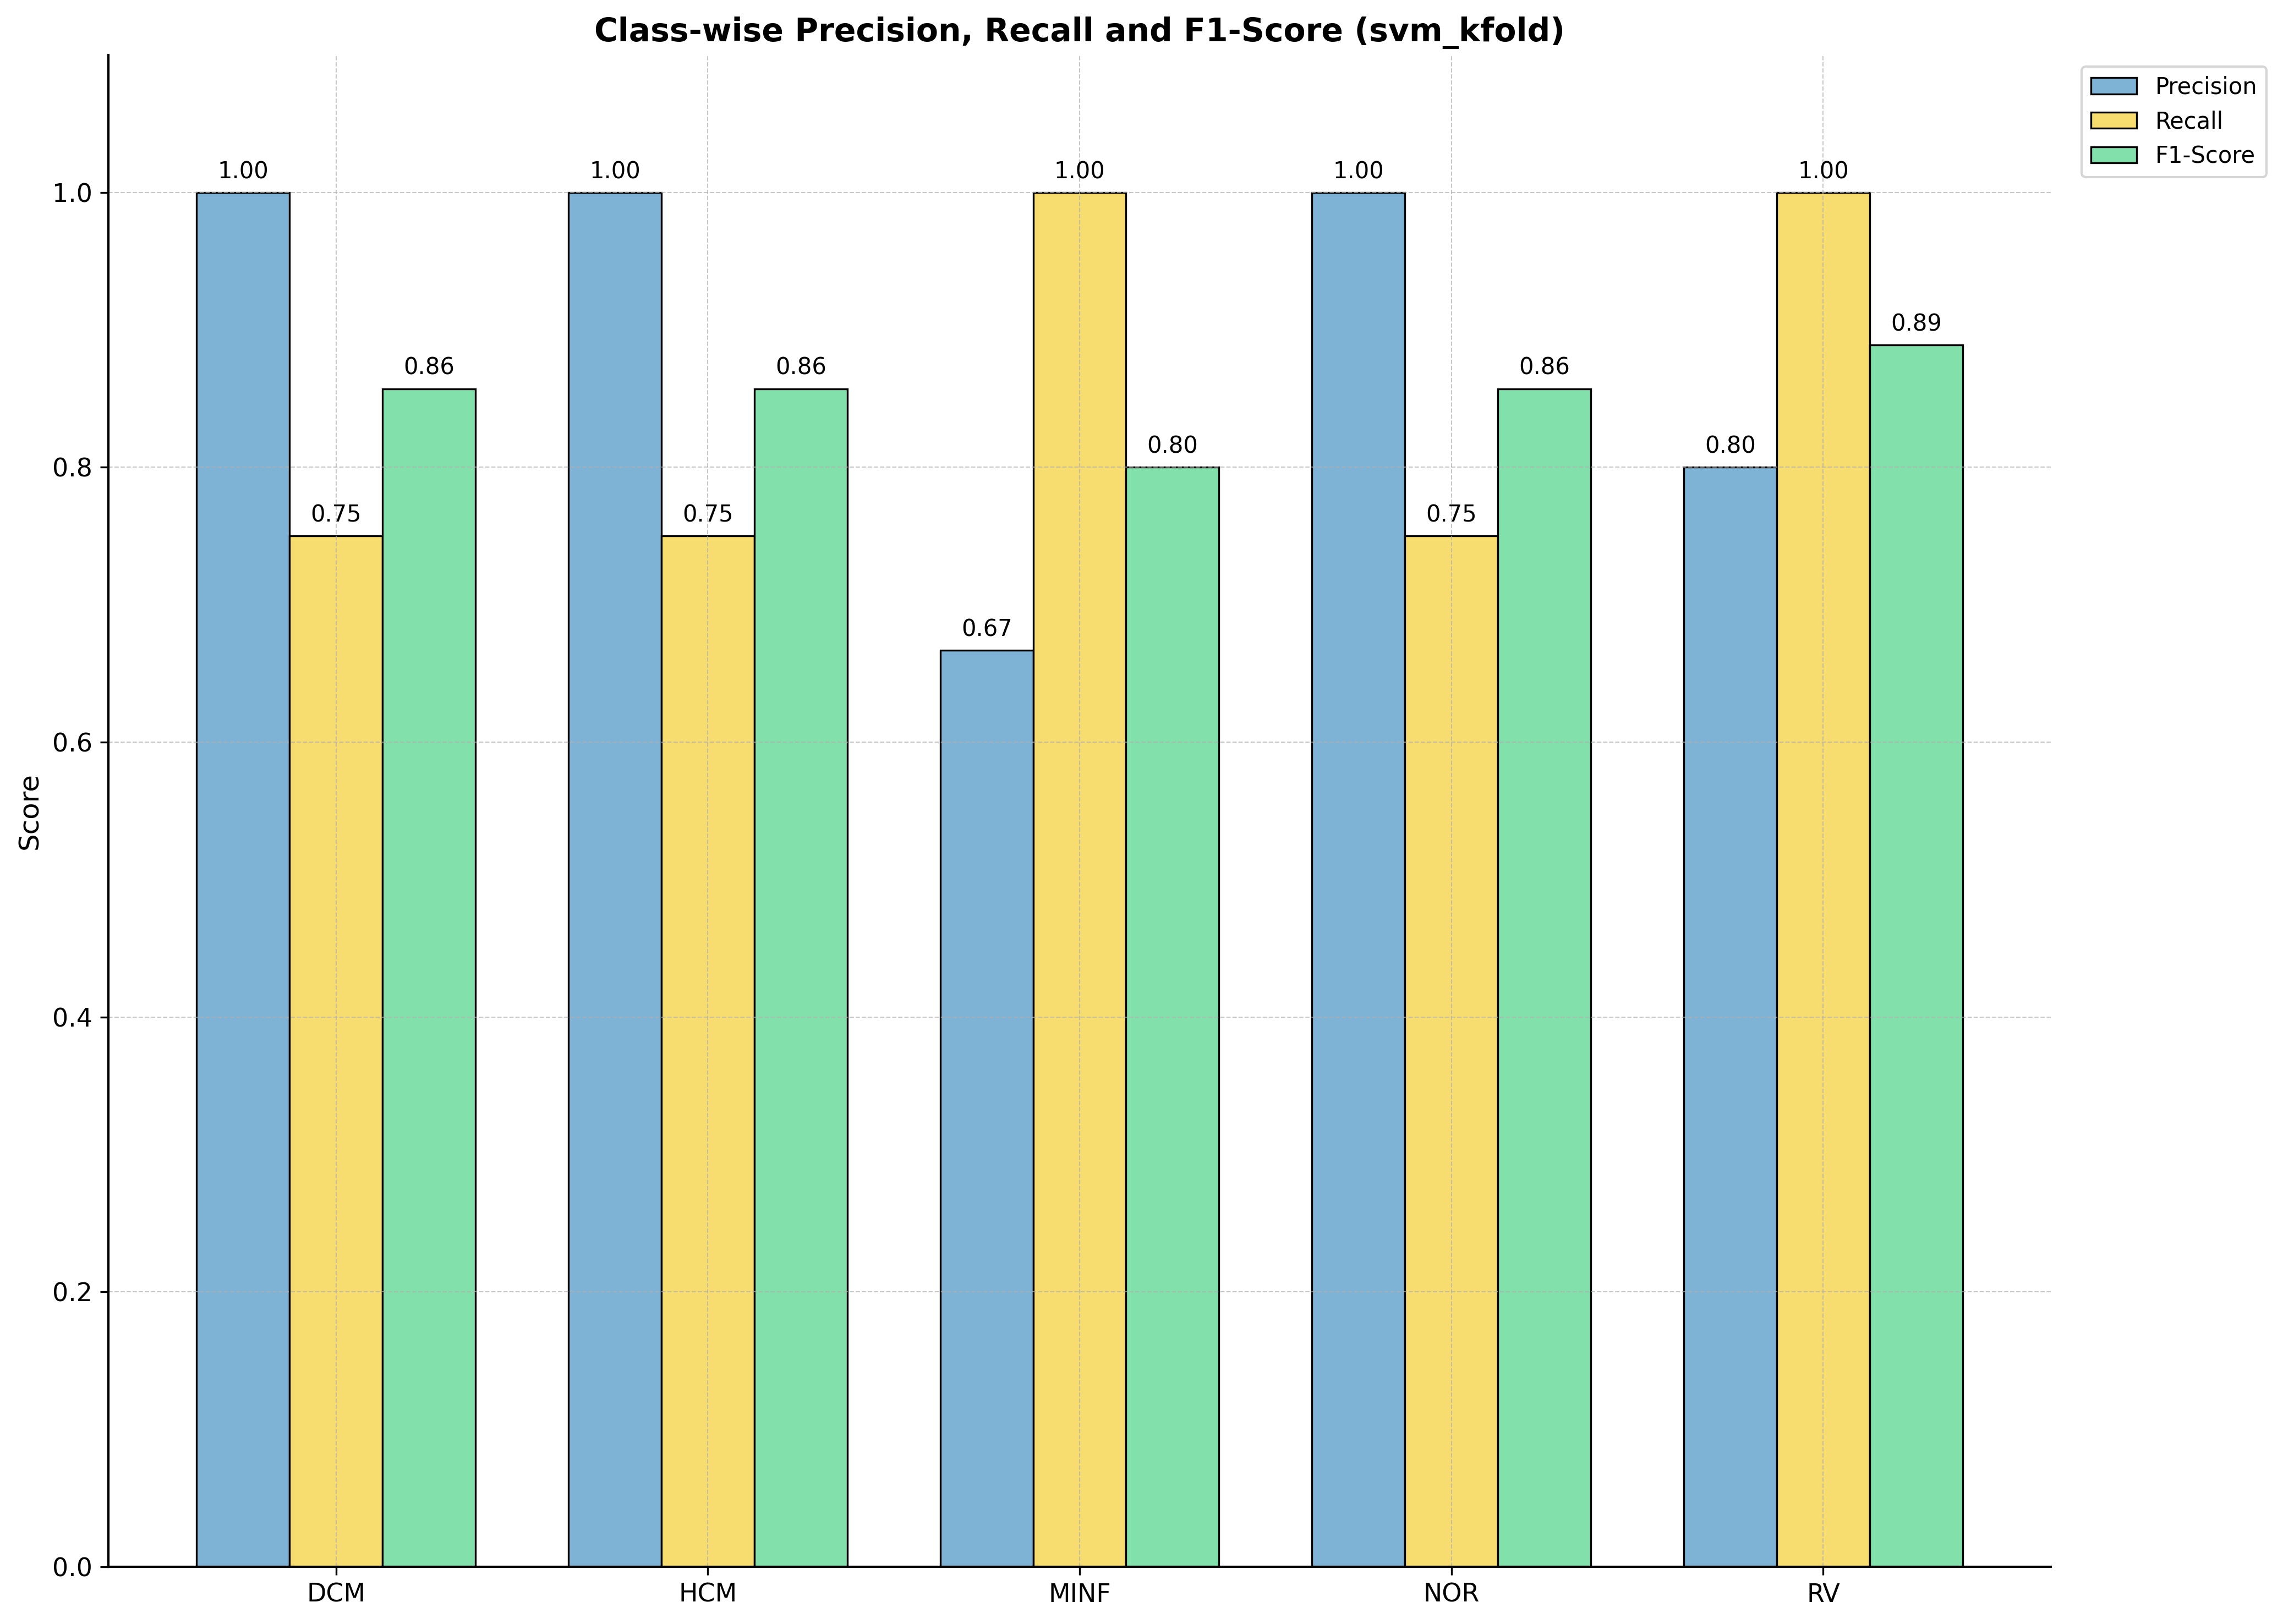
\includegraphics[width=0.99\textwidth]{../images/metrics/svm/svm_kfold_class_wise_metrics.png}
	\end{center}
	\caption{Class-wise Precision, Recall, and F1-Score for the Support Vector
		Machine (SVM) model trained with Stratified K-Fold cross-validation. DCM $=$
		Dilated Cardiomyopathy, HCM $=$ Hypertrophic Cardiomyopathy, MINF $=$
		Myocardial Infarction, NOR $=$ Normal, RV $=$ Right Ventricular abnormality.}
	\label{fig:fig4}
\end{figure}
